\documentclass[a4paper]{article}

\usepackage{graphicx}          % For including graphics.
\usepackage{amsmath}           % Some mathematical symbols.

\addtolength{\topmargin}{-20mm}% Margin adjustments.
\addtolength{\textheight}{20mm}% Margin adjustments.

\begin{document}

\title{Report Template for EQ2425 Analysis and Search of Visual Data\\

\large{EQ2425, Project X}} 

\author{Author 1\\ author1@x.com
  \and Author 2\\ author2@y.com}
% \date{March 17, 2009} % Manual date

\maketitle

\section*{Summary}
\label{sec:summary}

Write a short summary of your report. Write approximately 150 words about the
problem that you are considering, your solution, obtained results and the
the conclusion. For example, this template provides instructions for writing the
project reports for the EQ2425 Analysis and Search of Visual Data course. Read it thoroughly as it
is expected that the instructions are followed.

\section{Introduction}
\label{sec:introduction}

Give an introduction to the problem considered. The introduction should be
written such that it can be understood by an engineer whose area of expertise is
not image processing. Motivate the problem by using references to work by other
authors~\cite{coursebook}, as well as interesting applications.

Define the mathematical notation used in the report and state the problem using
this notation. Make sure that any assumptions you are using are explicit. It is
often convenient to be able to refer to equations by numbers. An example
equation is the additive noise degradation model for images
\begin{equation}
  \label{eqn:model}
  g(x,y) = f(x,y) + \eta(x,y).
\end{equation}

\section{Problem Description}
\label{sec:system}
Give a description of the system that is implemented for finding a solution to
the problem stated in~Section \ref{sec:introduction}. Any derivations that are
useful for understanding the solution are presented here. Describe and motivate
implemented algorithms.

\section{Results}
\label{sec:results}

To confirm your findings and the performance of your algorithms, present
simulation results in this section. All results should be explained in the text.
Plot your results in figures such as Figure~\ref{fig:histogram}, which shows the
histogram of~\eqref{eqn:model} for a given image $f(x,y)$ and
$\eta(x,y) = 0$.
\begin{figure}[!ht]
  \centering
  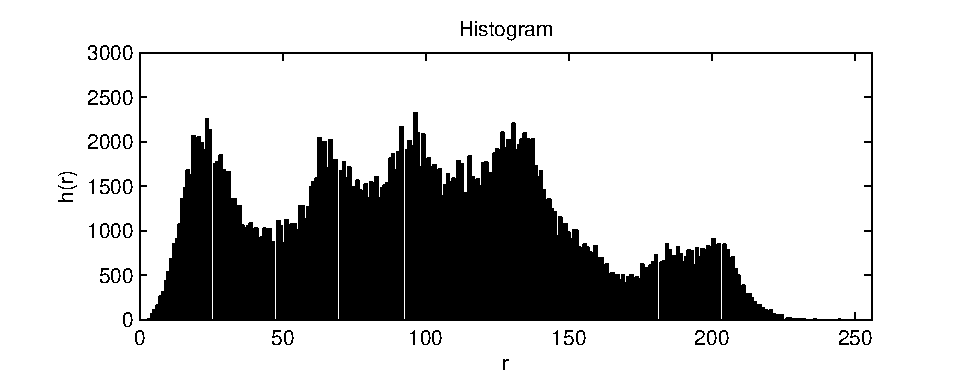
\includegraphics[width=0.9\columnwidth]{histogram.eps}
  \caption{Make sure to name the axis. In this figure the gray level is denoted
  $r$ and $h(r)$ is the number of pixels with gray level $r$.}
  \label{fig:histogram}
\end{figure}

Sometimes images give a better understanding of the obtained results.
Figure~\ref{fig:lena} gives a better description of $f(x,y)$ than
Figure~\ref{fig:histogram} for certain purposes. However, make sure that you
have a good motivation for the inclusion of any graphics. They should all aid
the reader in understanding your report.
\begin{figure}[!ht]
  \centering
  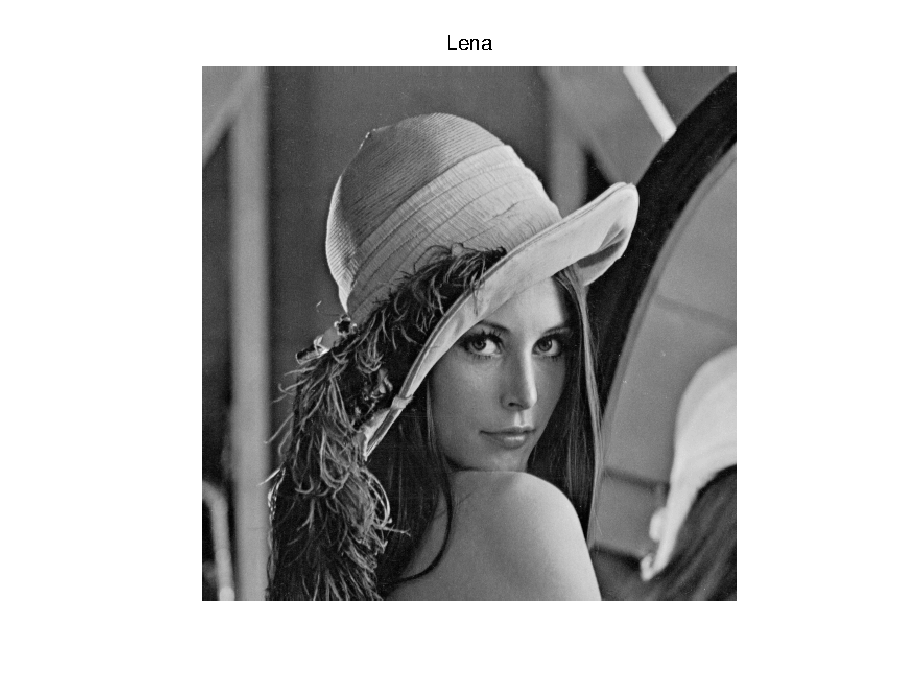
\includegraphics[width=0.9\columnwidth]{lena.eps}
  \caption{Each figure should be well explained in the caption, as well as in
  the text.}
  \label{fig:lena}
\end{figure}

\section{Conclusions}
\label{sec:conclusions}

Present your conclusions in this section. Remember that conclusions are not just
another summary. Your report, excluding references and appendix, should fit in
4-6 A4-pages. Therefore, make sure to write concisely and to the point,
describing everything of importance. Writing a report takes time, which is why
you should start early. If you have any questions about the assignment ask the
teaching assistants in time. Name your report pdf-file in the format
\verb\20YYpX_author1_author2.pdf\, where \verb\author1\ and \verb\author2\ are
surnames of the authors.

\section*{Appendix}

\subsection*{Who Did What}
Describe in detail how the project work was divided between the authors.
This template was written by Ermin Kozica in \LaTeXe. A good introduction to
\LaTeXe is available at~\cite{latexmanual}. You can write your report in other
programs as well.




\begin{thebibliography}{99}
\bibitem{coursebook} Rafael C. Gonzalez and Richard E. Woods,
  \textsl{Digital Image Processing},
  Prentice Hall, 2nd ed., 2002
\bibitem{latexmanual} Tobias Oetiker et al.,
  \textsl{The Not So Short Introduction to \LaTeXe},
  Available: http://tobi.oetiker.ch/lshort/lshort.pdf,
  Last accessed: March 17, 2009
\end{thebibliography}
\end{document}
